\documentclass[12pt, twoside]{article}
\usepackage[francais]{babel}
\usepackage[T1]{fontenc}
\usepackage[latin1]{inputenc}
\usepackage[left=7mm, right=7mm, top=7mm, bottom=7mm]{geometry}
\usepackage{float}
\usepackage{graphicx}
\usepackage{array}
\usepackage{multirow}
\usepackage{amsmath,amssymb,mathrsfs}
\usepackage{textcomp}
\pagestyle{empty}
\usepackage{soul}

\begin{document} 


\begin{center}
{\fbox{$4^{e}3$ \qquad \qquad \textbf{\Large{Devoir surveill� 4 }}
\qquad \qquad 28/01/2014}}
\end{center}

\bigskip


\ul{\textbf{Exercice 1}}: (\textit{3,5 points})

\enskip

\begin{tabular}{cc}
\begin{minipage}{16cm}
Sur la figure ci-contre, les droites (EF) et (BC) sont parall�les, AE=4,5cm,
EB=2,5cm, EF=2,7cm et AC=9,8cm. Calculer BC et AF. Justifier votre
r�ponse.


\end{minipage}
&
\begin{minipage}{25mm}

\end{minipage}
\end{tabular}

\bigskip




\ul{\textbf{Exercice 2}}: (\textit{4 points})


\enskip
 

\begin{tabular}{cc}
\begin{minipage}{12cm}
Odette, confortablement allong�e sur la plage d'Etretat, voit align�s le sommet
de son parasol O et celui des falaises S. 
On admettra que les falaises et le parasol sont en position verticale par
rapport � la plage horizontale. La t�te d'Odette T est � 1,60m du pied du
parasol P. Le parasol, de 1,40m de haut, est plant� � 112 m de la base des
falaises B.
\end{minipage}
&
\begin{minipage}{6cm}
\begin{center}
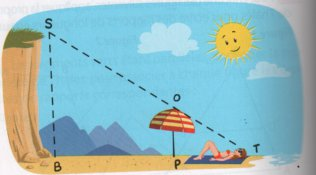
\includegraphics[width=6cm]{images/plage.jpg}
\end{center}
\end{minipage}
\end{tabular}

\begin{enumerate}
  \item Faire un sch�ma.
  \item Que peut-on dire des droites (SB) et (OP)? Justifier votre r�ponse.
  \item Calculer la hauteur BS des falaises. Justifier votre r�ponse.
\end{enumerate}

\bigskip




\ul{\textbf{Exercice 3}}: (\textit{3 points})

\begin{tabular}{cc}
\begin{minipage}{16cm}


Dans cette vue de profil d'un escabeau touchant le sol en deux points A et B,
la planche d'appui [CD] est parall�le � [AB], EA=2,40m, AC=2m et CD=0,25m.

D�terminer en justifiant et en d�taillant les calculs, la distance AB s�parant
les deux pieds de l'escabeau.
 
\end{minipage}
&
\begin{minipage}{25mm}
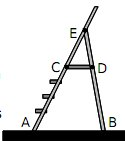
\includegraphics[width=25mm]{images/ex2.jpg}
\end{minipage}
\end{tabular}



\bigskip




\ul{\textbf{Exercice 4}}: (\textit{5,5 points})

\enskip

\begin{tabular}{cc}
\begin{minipage}{12cm}

 Sur la figure ci-contre, les droites (MN) et (BC) sont parall�les et AB=10cm.
 
 \begin{enumerate}
   \item Montrer que AC=8cm. Justifier votre r�ponse.
   \item Calculer BC. Justifier votre r�ponse.
   \item Montrer que le triangle ABC est rectangle.
   \item Calculer l'aire du quadrilat�re ABCD.
 \end{enumerate}
\end{minipage}
&
\begin{minipage}{6cm}
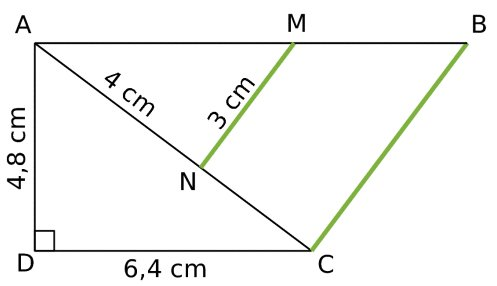
\includegraphics[width=6cm]{images/ex4.jpg}
\end{minipage}
\end{tabular}


\bigskip




\ul{\textbf{Exercice 5}}: (\textit{4 points})

\enskip

\begin{tabular}{cc}
\begin{minipage}{14cm}


 


En utilisant les informations port�es sur la figure, calculer les longueurs DF
et FH en justifiant vos r�ponses. (Les mesures sont en centim�tres.)

\end{minipage} 
&
\begin{minipage}{45mm}
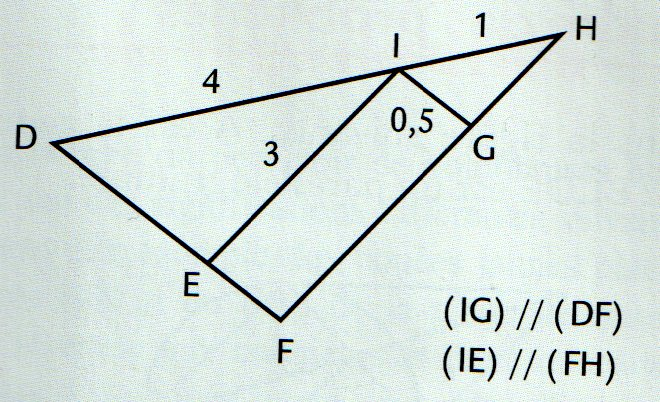
\includegraphics[width=45mm]{images/ex7.jpg}
\end{minipage}
\end{tabular}


\end{document}
